\section{Implementation Details}

\subsection{Objects}
\label{sec:object_model}
\algo\ models a variety of deformable objects of different dimensionalities, ranging from 0-dimensional  liquid, 1-dimensional rope, to 2-dimensional cloth. The underlying deformation and the dynamics vary distinctly for each dimension. In general, the lower the dimension is, the higher the degrees of freedom (DoFs) of the system, thus the more complex modeling that system becomes. 
We use two different representations to model the deformable objects to balance the modeling capacity with its complexity: water and rope are modeled using Material Point Method (MPM), while the cloth is modeled using a mass-spring system. 

\textbf{Modelling Water and Rope using MPM} Material Point Method (MPM) demonstrates strong modeling capacity and flexibility. MPM models the deformable objects as a set of particles; each particle is represented by its position and some properties such as mass. The dynamics and the deformation of the object are computed by simulating the interactions among all individual particles, conforming to some pre-defined physics rules. This Particle-level representation and the dynamics simulation allow MPM to model the object under severe deformation. We, therefore, choose to use MPM to model water and rope that can undergo severe deformation, for they can exploit the model capacity of MPM to its full potential.

\textbf{Modelling Cloth using Mass-Spring System} Cloth only undergoes limited deformation as it has to conform to the canonical shape of the initial cloth through manipulation. This limited deformable does not require the strong modeling capacity of MPM, which is computationally expensive. Therefore, rather than modeling the deformation on the Particle-level, we choose to model the cloth using the mass-spring system, which is a simpler model that uses the physical constraints as a prior. 



\subsection{Code Example}
\label{sec:code_example}

\definecolor{codegreen}{rgb}{0,0.6,0}
\definecolor{codegray}{rgb}{0.5,0.5,0.5}
\definecolor{codepurple}{rgb}{0.58,0,0.82}
\definecolor{backcolour}{rgb}{0.95,0.95,0.92}

\lstdefinestyle{mystyle}{
    backgroundcolor=\color{backcolour},   
    commentstyle=\color{codegreen},
    keywordstyle=\color{magenta},
    numberstyle=\tiny\color{codegray},
    stringstyle=\color{codepurple},
    basicstyle=\ttfamily\footnotesize,
    breakatwhitespace=false,         
    breaklines=true,                 
    captionpos=b,                    
    keepspaces=true,                 
    numbers=left,                    
    numbersep=5pt,                  
    showspaces=false,                
    showstringspaces=false,
    showtabs=false,                  
    tabsize=2
}

\lstset{style=mystyle}

\begin{lstlisting}[language=Python, caption=Example of Running Cloth Environment]
import numpy as np
from core.envs.registration import env_functions

env = env_functions["fold_cloth3"](batch_size=32, seed=1)
obs, state = env.reset(env.simulator.key_global)

actions = np.random.uniform(0, 1, (env.batch_size, env.action_size))
obs, reward, done, info = env.step_diff(actions, state)
\end{lstlisting}

\begin{lstlisting}[language=Python, caption=Example of Computing Action Gradients via \simulator]
import jax
import numpy as np
from core.envs.registration import env_functions

env = env_functions["fold_cloth3"](batch_size=32, aux_reward=True)
obs, state = env.reset(env.simulator.key_global)
actions = np.random.uniform(0, 1, (env.batch_size, env.action_size))

@jax.jit
@jax.grad
def compute_grad(actions, state):
    obs, reward, done, info = env.step_diff(actions, state)
    return -reward.sum()

print("action gradients", compute_grad(actions, state))
\end{lstlisting}

\subsection{Jax to parallelize}
\label{sec:jax}
One major limitation of the existing simulators is the lack of support for highly paralleled sampling. The key challenges for Deformable Object Manipulation are the complex governing equations and the enormous state space. The complex governing equations invalidate most of the analytical approaches since solving the complex governing equations is intractable. On the other hand, the success of the sampling-based methods hinges on the reasonable coverage of the state space. The lack of support for highly paralleled sampling to better cover the state space is a major impediment to the works on Deformable Object Manipulation. \algo\ fills in this gap by implementing its simulator using JAX, which supports highly paralleled sampling with great automatic differentiation. Using our implementation, we can finish an iteration (both forward and backward pass) for 128 rollouts with 80 timesteps on a server with 4 2080-Ti GPUs in 3 seconds.

\subsection{Saving Memory}
\label{sec:saving_memory}
\textbf{Lazy Dynamic Update} \algo\ optimizes the time and memory consumption of MPM by only updating the dynamic of a small region affected by the manipulation at each step. MPM models and updates the state and dynamics on the Particle-level; its time and memory consumption is proportional to the size of the environment, which can be arbitrarily large. Our insight is that, though the deformable object can potentially interact with the entire environment, only a small region will be affected at each time. 
This inspires \algo\ to optimize the time and memory consumption of running MPM by exclusively considering the \textit{active region} during the interactions. Using this trick, \algo\ effectively reduces the computation time by two orders of magnitude on average. Taking the rope for example, the original environment is of size $128 \times 128 \times 128$. However, a grid of size $32 \times 6 \times 32$ is sufficient to cover the region of interaction between the environment and the rope. Therefore, we first detect the \textit{active region} of size $32 \times 6 \times 32$, then we perform a linear transformation to shift the \textit{active region} to the \textit{origin}, perform the update due to deformation and interaction, finally we shift the updated \textit{active region} to align with its original coordinates.

\begin{figure}
\centering
\subcaptionbox{Detect the active region.}{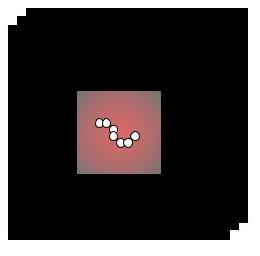
\includegraphics[width=0.2\columnwidth]{figs/MPM_speedup/active_region.jpg}}
\hspace{50pt}
\subcaptionbox{Update the deformation.}{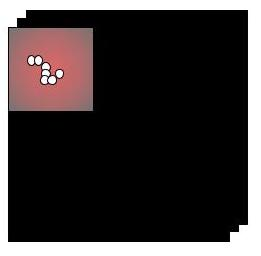
\includegraphics[width=0.2\columnwidth]{figs/MPM_speedup/shift_up.jpg}}
\hspace{50pt}
\subcaptionbox{Shift back the update active region.}{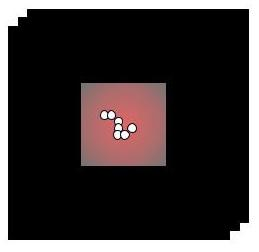
\includegraphics[width=0.2\columnwidth]{figs/MPM_speedup/shift_back.jpg}}
\caption{
We demonstrate how to use the active region to reduce the computation complexity for the simulation. Taking rope for example, the original environment, denoted as the black background, is of size $128 \times 128 \times 128$, while the active region, where the region that will be actively changed due to the current deformation highlighted in red, is of size $32 \times 6 \times 32$, as illustrated in (a). To avoid updating all the particles in the environment, in ( b), we shift the active region to the top corner, the \textit{origin} of the environment, and update the dynamic and observation. Finally, in ( c), we shift the updated active region back to align its original coordinates.}
\label{fig:MPM_speedup}
\end{figure}

\textbf{Checkpointing method} \algo \ only stores the values of a few states (i.e. checkpoints), and re-evaluates the sub-step gradients online during the back-propagation to reduce the memory consumption for long horizon problems. The checkpointing method has been proven useful in saving the memory consumption for differentiable simulations in many prior works \citep{checkpoint, chen_checkpoint, Griewank_checkpoint}.
To make the simulator end-to-end differentiable, every value in the neural network that is computed during the forward pass has to be saved, as they are needed to compute the gradient during the backward pass. The computation complexity scales up quickly w.r.t. the length of the task horizon. This is a significant problem for our simulator for high DoFs deformable object manipulation, as the memory required for each timestep's update is enormous compared to its rigid body counterpart. 
To overcome the large memory consumption issue, \algo\ trade-offs the computation complexity slightly for large memory consumption improvement: \algo\ only stores the values of a few states (i.e. checkpoints) at the forward pass; during the backward propagation, \algo\ re-compute segments of the forward values starting from every stored state in the reverse order sequentially for the overall gradient.
With this trick, \algo\ now doubles the computation complexity, but saves an arbitrary amount of memory, depending on the intervals of the states saved. 

\subsection{Discontinuous Gradient}

As an end-to-end differentiable simulator, the effectiveness of \algo\ rests on the accuracy of the gradient computed. We found that for deformable object manipulation, the action not in contact with the object will cause the gradient to be discontinuous, which causes the estimate of the gradient after this action to suffer from high variance and poor accuracy in the backward propagation. To mitigate this problem, for every action input by the agent or the human user, \algo\ will perform local adjustment such that the action will always make the gripper in contact with the deformable objects. This ensures that our gradient is end-to-end continuous therefore improving the accuracy of the estimated gradient.

